

\noindent\textbf{11. (CRLS 22.3-10)} Mostre como um vértice $u$ num grafo orientado pode terminar sozinho numa árvore de uma floresta \proc{DFS} mesmo tendo arcos saindo e entrando dele em $G$.

A figura \ref{fig:7.11-1} mostra um exemplo onde o vértice $u$ pode ficar sozinho numa árvore de uma floresta \proc{DFS} gerada a partir do vértice $s$.
\begin{center}
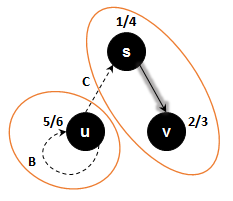
\includegraphics[width=0.33\textwidth]{q7-11-p1.png}
\captionof{figure}{Exemplo onde o vértice $u$ pode ficar isolado.}
\label{fig:7.11-1}
\end{center}


Um outro exemplo pode ser visto na figura \ref{fig:7.11-2}, sendo que cada árvore é formada por um único vértice, já que a busca começa em $v$.
\begin{center}
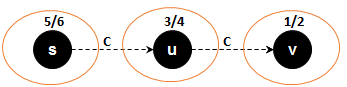
\includegraphics[width=0.48\textwidth]{q7-11-p2.png}
\captionof{figure}{Segundo exemplo onde o vértice $u$ pode ficar isolado.}
\label{fig:7.11-2}
\end{center}